\documentclass[12pt]{article}
\usepackage[paper=letterpaper,margin=2cm]{geometry}
\usepackage{amsmath}
\usepackage{amssymb}
\usepackage{amsfonts}
\usepackage{newtxtext, newtxmath}
\usepackage{enumitem}
\usepackage{titling}
\usepackage{graphicx}
\usepackage[colorlinks=true]{hyperref}

\setlength{\droptitle}{-6em}

\title{Stat 61 final with solutions}
\date{}

\begin{document}
\maketitle
\vspace{-2cm}
\noindent {\bf Name:} $\rule{8cm}{0.5mm}$
\vspace{1cm}

\noindent {\bf Swat ID/Username:} $\rule{6cm}{0.5mm}$
\vspace{-0.5cm}

\section*{Version 1}
\subsection{True/False}
Circle either True or False for each statement. Make sure you read each statement carefully! (2 points each)
\begin{enumerate}[leftmargin=\labelsep]
\item {\bf True \hspace{3mm}or\hspace{3mm} False}\hspace{4mm} The maximum likelihood estimator is always unbiased. \vspace{3mm} 
\item {\bf True \hspace{3mm}or\hspace{3mm} False}\hspace{4mm}  A p-value is a probability evaluated under the assumption that the null hypothesis\\ $\hspace*{3.5cm}$ is correct. %\vspace{mm}\\ 
\item {\bf  \hspace{3mm}or\hspace{3mm} False}\hspace{4mm}  A random variable $U\sim Unif(0,\theta)$, where $\theta>0$ has a probability distribution that\\ $\hspace*{3.5cm}$ belongs to the one parameter exponential family.     
\vspace{3mm} 
\item {\bf True \hspace{3mm}or\hspace{3mm} }\hspace{4mm}  They Neyman-Pearson Lemma implies that we can find a uniformly most powerful\\ $\hspace*{3.5cm}$ test for $H_0: \theta = \theta_0$ vs $H_1: \theta > \theta_0$, where $\theta$ is the probability of a positive outcome\\ $\hspace*{3.5cm}$ for a random variable following a $Bin(n, \theta)$ distribution.     
\vspace{3mm} 
\item {\bf True \hspace{3mm}or\hspace{3mm} False}\hspace{4mm}  A Bayes' estimate for a parameter $\theta$ is always consistent.     
\vspace{3mm} 
\item {\bf \hspace{3mm}or\hspace{3mm} False}\hspace{4mm}  The lower and upper bounds of a confidence interval are fixed (deterministic)\\ $\hspace*{3.5cm}$ whereas the lower and upper bounds of a (Bayesian) credible interval are random.     
\vspace{3mm} 
\item {\bf  \hspace{3mm}or\hspace{3mm} False}\hspace{4mm}  If a $95\%$ confidence interval for $\theta$ includes the value where $\theta=3.2$, then an $\alpha=0.01$\\ $\hspace*{3.5cm}$ level significance test of $H_0: \theta = 3.2$ vs $H_1: \theta \neq 3.2$ will fail to reject the null.     
\vspace{3mm} 
\item {\bf True \hspace{3mm}or\hspace{3mm} }\hspace{4mm}  An ANOVA test compares the means of different groups in a population.    
\vspace{3mm} 
\item {\bf  \hspace{3mm}or\hspace{3mm} False}\hspace{4mm}  A Chi-square Test of Homogeneity compares the means of different populations.     
\vspace{3mm} 
\item {\bf True \hspace{3mm}or\hspace{3mm} False}\hspace{4mm}  If an estimator is consistent, then it is also unbiased.     
\end{enumerate}


\subsection{Multiple Choice}
Circle the best answer from among the options provided for each question. (3 points each)\\


\noindent For Questions 1-7 consider each problem setting and determine which procedure to use to answer the research question. 

\begin{enumerate}[leftmargin=\labelsep]
\item A textile engineer is interested whether the mean breaking strength of Yarn Type A is larger than that of Type B. \\ \vspace{1mm}\\
{\bf (a)} \hspace{2mm} {\bf An independent two-sample t-procedure}\\  \vspace{1mm}\\
{\bf (b)} \hspace{2mm} Paired two-sample t-procedure\\   \vspace{1mm}\\
{\bf (c)} \hspace{2mm} Chi-square test for independence\\  \vspace{1mm}\\
{\bf (d)} \hspace{2mm} Chi-square test for homogeneity\\

\item Researchers want to test a new theory in parasitology which states that the mean yield of an entozoic amoebae is consistent across four different treatment conditions.\\ \vspace{1mm}\\
{\bf (a)} \hspace{2mm} Chi-square test for independence\\ \vspace{1mm}\\
{\bf (b)} \hspace{2mm} Chi-square test for goodness-of-fit\\   \vspace{1mm}\\
{\bf (c)} \hspace{2mm} Chi-square test for homogeneity\\  \vspace{1mm}\\
{\bf (d)} \hspace{2mm} {\bf An ANOVA procedure}\\  

\item  Historians review a data set of the passengers aboard the RMS Titanic which famously sunk after crashing into an iceberg in the Atlantic in 1912. They are interested in whether the class of people aboard the ship played a role in whether someone survived the crash. People onboard were divided into four class categories: crew members, 1st class, 2nd class, and 3rd class.\\ \vspace{1mm}\\
{\bf (a)} \hspace{2mm} Paired two-sample t-procedure\\ \vspace{1mm}\\
{\bf (b)} \hspace{2mm} {\bf Chi-square test for independence}\\   \vspace{1mm}\\
{\bf (c)} \hspace{2mm} An ANOVA procedure\\  \vspace{1mm}\\
{\bf (d)} \hspace{2mm} An independent two-sample t-procedure\\

\item A political scientist conducts a local study to determine whether voter turnout rate is associated with political party affiliation. They survey a random selection of county residents with sample sizes relative to the proportion of the registered Democrat, Republican, and third party voters, that is, 43\%, 48\%, and 9\%, respectively, and the record whether or not each individual voted in the last election.\\ \vspace{1mm}\\
{\bf (a)} \hspace{2mm} Chi-square test for homogeneity\\ \vspace{1mm}\\
{\bf (b)} \hspace{2mm} Chi-square test for independence\\   \vspace{1mm}\\
{\bf (c)} \hspace{2mm} An ANOVA procedure\\  \vspace{1mm}\\
{\bf (d)} \hspace{2mm} {\bf Chi-square goodness-of-fit procedure}\\

\item A veterinarian conducts a study on nine randomly selected cats and records the average daily water intake for each each cat when exposed to sill water or flowing water for four days. Each cat is randomly assigned two days under each water condition. On average, how much more water will cats drink from a flowing water source compared to a still water source?\\ \vspace{1mm}\\
{\bf (a)} \hspace{2mm} {\bf Paired two-sample t-procedure}\\ \vspace{1mm}\\
{\bf (b)} \hspace{2mm} An independent two-sample t-procedure\\   \vspace{1mm}\\
{\bf (c)} \hspace{2mm} Chi-square test for homogeneity\\  \vspace{1mm}\\
{\bf (d)} \hspace{2mm} Chi-square test for independence\\

\item In a study on the average length of hospital stay (in hours) for patients admitted to a local emergency room, patients are grouped into one of four different annual income levels: less than $\$20$K, between $\$20$K and $\$40$K, between $\$40$K and $\$80$K, and $\$80$K or more. The researchers want to determine if the average length of hospital stay is consistent across all four income brackets.\\ \vspace{1mm}\\
{\bf (a)} \hspace{2mm} Paired two-sample t-procedure\\ \vspace{1mm}\\
{\bf (b)} \hspace{2mm} {\bf An ANOVA procedure}\\   \vspace{1mm}\\
{\bf (c)} \hspace{2mm} Chi-square test for independence\\  \vspace{1mm}\\
{\bf (d)} \hspace{2mm} Chi-square test for homogeneity\\

\item A company wants to determine if sending a daily notification to their app users increases customers time spent on their app. They randomly select $500$ of their app users and randomly assign half of the users to receive a daily notification. The average time each individual interacts with the app is recorded and compared after two weeks of the treatment.\\
\vspace{1mm}\\
{\bf (a)} \hspace{2mm} Chi-square test for homogeneity\\ \vspace{1mm}\\
{\bf (b)} \hspace{2mm} Paired two-sample t-procedure\\   \vspace{1mm}\\
{\bf (c)} \hspace{2mm} {\bf An independent two-sample t-procedure}\\ \vspace{1mm}\\  
{\bf (d)} \hspace{2mm} Chi-square test for independence\\
\end{enumerate}



\noindent For Questions 8-10 suppose we have a sample of $X_1,\dots,X_n \stackrel{IID}{\sim} Exp(1/\theta)$ data points and we want to test $H_0: \theta=3$ vs $H_1: \theta=5$ at the $\alpha=0.02$ significance level. This test rejects for large values of $T(x_1, \dots, x_n) = \sum_{i=1}^{n}x_i$. Answer the next few questions based on the image below. 


\begin{figure}[h]
\centering
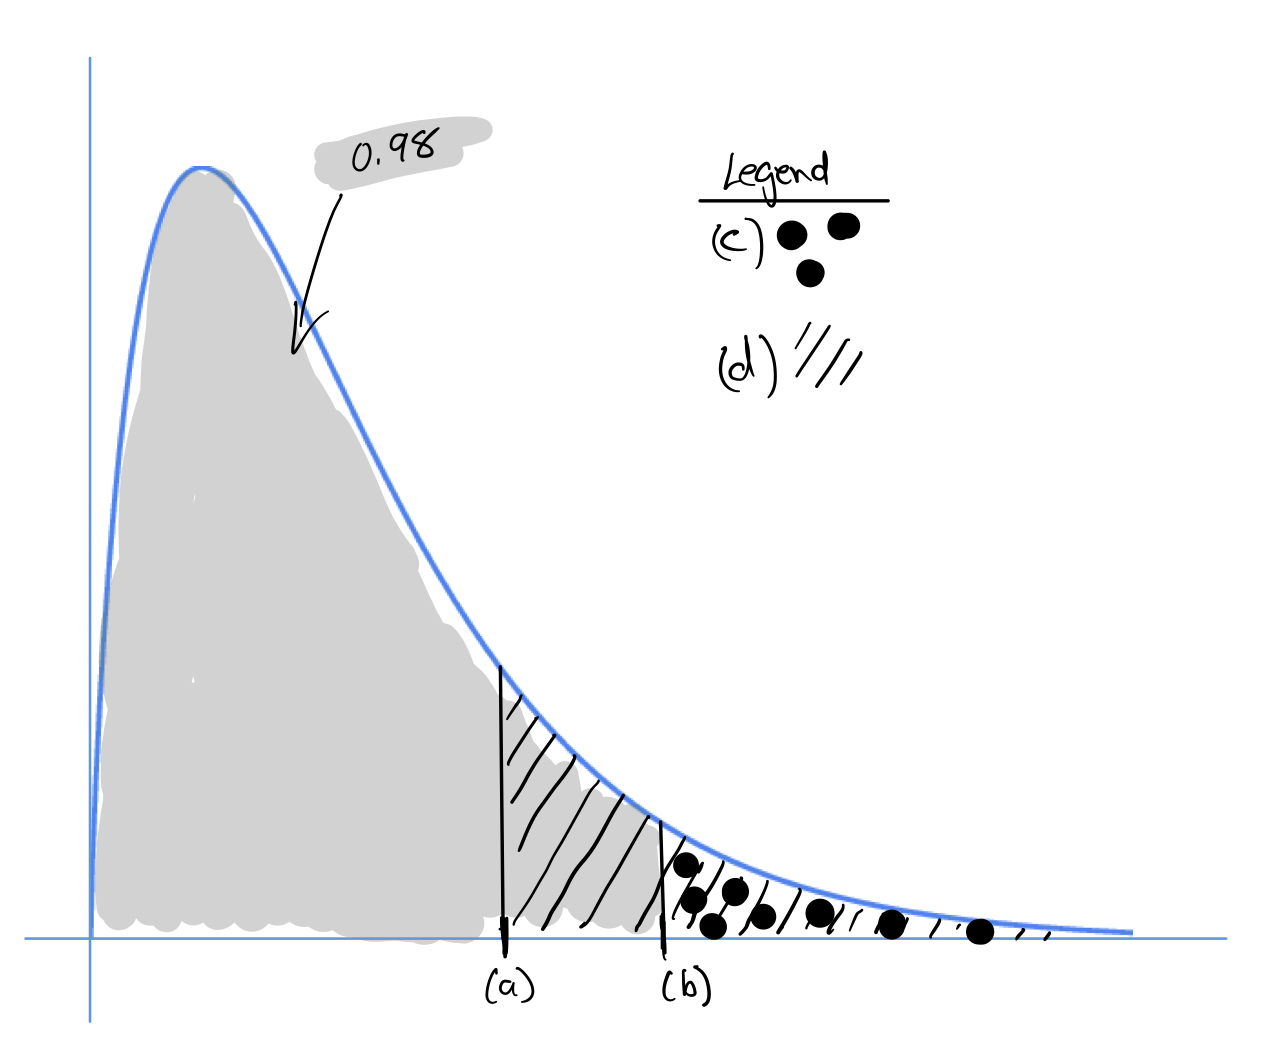
\includegraphics[width=0.7\linewidth]{Stat 61 final.png}
\end{figure}	

\begin{enumerate}[leftmargin=\labelsep]
\setcounter{enumi}{7}
\item Which label corresponds to the significance level?\\
\vspace*{.5cm}\\
\hspace*{1cm}(a) \hfill {\bf (b)} \hfill  (c) \hfill (d)\hspace*{1cm}\\
\vspace*{.5cm}\\

\item Which label corresponds to the observed test statistic?\\
\vspace*{.5cm}\\
\hspace*{1cm}{\bf (a)} \hfill (b) \hfill (c) \hfill (d)\hspace*{1cm}\\
\vspace*{.5cm}\\

\item Which label corresponds to the p-value?\\
\vspace*{.5cm}\\
\hspace*{1cm} (a) \hfill (b) \hfill (c) \hfill {\bf (d)}\hspace*{1cm}\\
\vspace*{.5cm}\\
\end{enumerate}

\subsection{Free Response}
Answer the following questions and make sure you show your work and/or explain your reasoning. Please label any work that does not fit in the space below and hand that in with your test. 
\begin{enumerate}[leftmargin=\labelsep]
\item Apply the factorization theorem to find the sufficient statistics of $X_1, \dots, X_n \stackrel{IID}{\sim} Beta(a, b)$. \textcolor{blue}{Hint: simplify as much as possible, may not look very simple} (6 points)
\pagebreak 

\item Given an IID sample of data $X_1, \dots, X_n$ from an $Exp(\theta)$ distribution, answer the two questions below.\\

(a) What is the posterior distribution for $\theta$ if we use a uniform prior, $\pi(\theta) \sim Unif(0,1)$? (4 points) \textcolor{blue}{Don't both evaluating the integral}\\
\vspace{5in}\\
(b) What is the method of moments estimator for $\theta$? (4 points)\\
\pagebreak 

%\item Show that estimator for $\theta$ is consistent. (6 points)\\
%\vspace{3cm}

\item Suppose we have a sample of IID data, $X_1, \dots, X_n$ from a $\chi^2_{(\nu)}$ distribution. What is the uniformly most powerful test for $H_0: \nu = 1$ vs $H_0: \nu >1$? (Provide both your test statistic and rejection region as explicitly as possible.) \textcolor{blue}{Hint: won't be able to find explicit solution for quantile, make sure defined completely. }(8 points)\\
\pagebreak 

\item Suppose $U \sim \chi^2_{\nu_1}$ is independent of $V \sim \chi^2_{\nu_2}$.\\

(a) What is the likelihood for $\nu_1$? (5 points)\\
\vspace{3in}\\
(b) Let $W = \frac{U/\nu_1}{V/\nu_2}$. What is the likelihood for $(\nu_1, \nu_2)$ given  $W = w_{obs}$? (5 points) \textcolor{blue}{Hint: give form of pdf for $Z=X/Y$ from Ch 3, answer should be written in terms of $w_{obs}$}\\
%Let $Y = \frac{\sum_{i=1}^{n} {W_i}/n}{\sum_{j=1}^{m}V_j/m} = \frac{U}{X}$. What is the likelihood for $Y$? (6 points)\\
\pagebreak 
%\item Suppose we choose an $\alpha = 0.02$ significance level for the test in Problem X above. What is the power of the test? (Your answer doesn't have to be a number but you should draw a picture or somehow indicate what calculation you would need to do to find the answer.\\
%\vspace{3cm}

\item In the simple linear regression mode we assume $$Y_i = \beta_0 + \beta_1 x_i + \epsilon_i, \quad \text{where} \epsilon \stackrel{IID}{\sim} N(0, \sigma^2).$$
Answer the following questions about estimators for parameters of this model. \textcolor{blue}{For simplicity, assume $\beta_0 = 0$}\\

(a) What is $\hat{\beta}_{1, MLE}$, i.e. the maximum likelihood estimator for $\beta_1$? (5 points)\\
\vspace{3in}\\
(b) What is the exact (finite) sample variance of $\hat{\beta}_{1, MLE}$? (5 points)\\
\vspace{3in}\\
(c) What is the large sample, asymptotic variance of $\hat{\beta}_{1, MLE}$? \textcolor{blue}{Hint: use score function and Fisher's info}(8 points)\\

\end{enumerate}





\end{document}
